
\newrefsection

%\textbf{B1.a. Extended Synopsis of the scientific proposal}

\chapter{B1.a. Extended Synopsis of the scientific proposal}\label{part1}

\eu{(max 5 pages)}

\eu{The Extended Synopsis should give a concise presentation of the scientific
proposal, with particular attention to the ground-breaking nature of the
research project and the feasibility of the outlined scientific approach.
Describe the proposed work in the context of the state of the art of the field.
References to literature should also be included. References do not count
towards the page limits. It is important that this extended synopsis contains
all essential information including the feasibility of the scientific proposal
since the panel will only evaluate Part B1 at step 1.}

\section{Long-term vision and ground-breaking nature of the project}

\subsection{Core contribution and impact}

AI and robots are emerging as key factors to successfully address modern societal
challenges, like the ageing society or increasing social isolation. In this
context, researchers in social robotics have the prime responsibility to ensure
that robots can understand and reason about their spatial and social environment
in such a way as to ensure a responsible and positive societal impact.

The basic idea of \emph{social robots} refers to robots that are situated in a
human social environment. In this context, we expect social robots to exhibit
\emph{social awareness}, i.e. to appraise and maintain a model of the social
situation in which they are embedded. Depending on the role of the robot, this
might include understanding who is present, who is interacting with whom, which
are the resulting groups,  what are the in-group roles,  etc.

Social awareness, as a socio-cognitive skill, is essential for the robot to e.g.
act in a context-sensitive manner; reason and apply social norms (for instance,
do not navigate in the middle of a group, or do not suddenly interrupt a
conversation); or create proactive social agents (in order to acknowledge and
respond to a human who would like to engage with the robot, the robot must first
adequately model and recognise the corresponding social situation).


\begin{figure}[H]
    \centering
    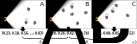
\includegraphics[width=0.9\linewidth]{figs/social-embeddings}
    \caption{General principle of social embeddings: arbitrary social situations
    are projected into real-valued vector space, \emph{embedding} their
    semantics. In this example (and assuming the perspective of the yellow
    character), scenes A and B  are more similar to each others (one person walking towards the
    character, with an independent group of people chatting in the background),
    than B and C (in C, the character is already engaged in an interaction).
    Social embeddings make it possible to compare such social situations using
    a simple distance between vectors.}
    \label{fig:social-embeddings}
\end{figure}

This can only be achieved if robots are endowed with the ability to represent
not only their physical environment, but also their social environment and
context. The \project project aims at designing, implementing and characterising
a radically novel method to achieve this goal, based on the concept of
\emph{embedding}: a low-dimensional, semantics-preserving, mathematical
representation of a high-dimensional input (Figure~\ref{fig:social-embeddings}).
Starting from a proof-of-concept of \emph{social embeddings} that I recently
published~\cite{lemaignan2024social}, \project develops and fully characterise
the concept of \emph{social embeddings}, that applies, for the first time, the
idea of building a compact numerical representation to the complexity of social
interactions and social dynamics.


At a scientific level, 
\TODO{articulate scientific impact}

Finally, \project is also about asserting and reinforcing the European
leadership in AI and intelligent robotics, in line with EU strong societal
values: a physical AI system able to represent and reason about its social
environment is also a system that can be designed to have an acceptable and
positive social impact, in line with the European objectives for socially
responsible AI. \project can directly contribute to these goals: the science and
technology that underpins the project \textbf{provide an important contribution
in securing a safe and responsible digital future in Europe}, as well as
\textbf{\project building the capacity in Europe to develop socially intelligent
embodied AI systems}. 


\subsection{Structure of the research programme}

\project is built around three axes: a basic research programme; an experimental
programme that looks specifically at the application of social embeddings to
social robotics; and, running in parallel to those first two axes, a scientific
investigation of the ethical dimension of social embeddings.

At the basic research level, \project targets the following
two overarching research goals: (1) build compact, yet semantics-preserving,
embeddings to represent arbitrary social and spatial environments for service
robots; fully characterize these embeddings, including their latent semantics;
(2) precisely frame the \emph{social awareness} enabled by social embeddings,
and demonstrate the key novel socio-cognitive capabilities that they enable.

I translate these two goals into six operational research objectives:

\begin{center}
    
\includegraphics[trim=0 0 0 0, clip,width=0.3\linewidth]{objectives}
\end{center}

\begin{enumerate}[label=\textbf{O\arabic*}]
    \item \label{T1} acquire and analyse a large dataset of real-world human
        interactions to identify a set of prototypical
        social situations; these will serve both for embedding fine-tuning, and
        as reference to analyse the topology and latent semantics of the social
        embedding space;

    \item \label{T2} study social dynamics by characterizing the trajectories of
        on-going social situations in the embedding space. I will look in
        particular into trajectories \emph{discontinuties}, that might represent
        unexpected changes of social dynamics, possibly a predictor of
        interaction failures, and social situation predictions, by extrapolating
        trajectories in the embedding space;

    \item \label{T5} because social embeddings also lend themselves to encoding
        task and social \emph{context} by simply attaching textual descriptions
        of the context, they open new possibilities for
        \emph{context-aware} representation and behaviour selection;


    \item \label{T3} as vector representations, social encodings lend
        themselves well to many downstream machine learning tasks
        that I will explore. For instance automatic engagement
        detection or socially-appropriate behaviour generation using Generative
        Adversarial Networks;

    \item \label{T4} contextualised lifelong adaptation of the robot's
        behaviours, by augmenting existing interactive machine learning
        techniques (`user in-the-loop' social learning, that I pioneered in
        social robotics\cite{senft2017supervised,
        winkle2020couch,winkle2021leador}) with representations of the social
        environment;

    \item \label{T6} finally, and because the development of
        socially-intelligent robots has complex ethical ramifications --
        including the potential of alienating human users --, \project also
        includes a strong research component on Responsible Robotics. In
        particular, the project will aim to contribute directly to the roadmap
        for Responsible Robotics, specifically investigating the interplay between
        machine learning applied to social robotics, transparency and human agency.

\end{enumerate}

These six objectives are reflected in the work package structure of the project,
presented in the next section.


\section{Feasibility of the project}


\subsection{Expertise and Research team}
\label{research-team}

My expertise is primarily centered on cognitive robotics and human-robot social
interaction. My expertise in this field covers a broad spectrum, from basic
research (for
example~\cite{lemaignan2014dynamics,lemaignan2015mutual,irfan2018social,winkle2019effective,bartlett2019what}),
to technical contributions (for instance~\cite{lemaignan2010oro,
lemaignan2017artificial, lemaignan2018underworlds})
to extensive experimental work (for instance~\cite{hood2015cowriter,winkle2020couch,
lemaignan2022social}).

Over the last 4 years, I have re-focalised my work on \emph{data-driven HRI},
contributing several new large datasets of social
interactions~\cite{lemaignan2018pinsoro,sallami2020unexpected,webb2023sogrin},
developing new data analysis
techniques~\cite{bartlett2019what,webb2022measuring}, and demonstrating with my
students new applications of interactive machine learning to social
interactions~\cite{senft2016sparc,winkle2020couch,winkle2021leador}.
In parallel, I progressively matured the idea of computing compact
\emph{embeddings} of social situations, until I published in 2023 a first
breakthrough in that direction~\cite{lemaignan2024social}. This ERC project is
directly born from this multi-year endeavour towards data-driven HRI, and aims
at significantly accelerate research in this direction.

In particular, \project is the opportunity to gather an interdiscplinary team of
academics that would effectively complement my expertise, and ensure the
feasibility of the project.

Specifically, I intend to recruit:

\begin{itemize}

    \item  two researchers with expertise in sociology and/or data-driven
        sociology (one senior post-doc PD1, one PhD student PHD1); these researchers will
        directly contribute to the human data acquisition and the interpretation
        of social embeddings in term of social situations;

    \item two researchers with expertise in large language models (one senior
        post-doc PD2, one PhD student PHD2); these researchers will contribute to the
        core implementation of social embeddings, including language model
        fine-tuning, as well as the analysis of the embedding space topology;

    \item one research in cognitive robotics (PhD student, PHD3); this research
        will focus on the integration of social embeddings into a larger
        cognitive architecture for social robots, able to autonomously drive
        interactions;

    \item one researcher with expertise in ethics of technology (post-doc
        level PD3); this researcher will lead the work on understanding social
        embeddings in terms of ethical and responsible research.
\end{itemize}

In addition, the host institution (INRIA Grenoble) will provide extensive
experience on machine learning applied to robotics. I will specifically build on
my already established collaboration with Dr. Xavier Almeida-Pineda, head of the
RobotLearn research group. Dr. Almeida-Pineda is the coordinator of the EU H2020
SPRING project on social robotics for geriatric care, and I am currently
Principal Investigator at PAL Robotics on this project).

Additional expertise, as well as access to experimental settings, will be
provided through a collaboration with Paris' public hospitals (APHP) and
specifically, with Dr. Maribel Pino, head of research at Paris' Broca hospital.

\subsection{Feasibility of the experimental program}

The experimental program is usually the more complex to run. For \project, it
relies on (1) having the requested AI software ready; (2) implementing the AI
software on an actual robotic platform; (3) deploy the robot in real-world
public spaces, with the associated practical know-how.

Regarding item (1): using publicly available resources, including machine learning architectures
like Transformers, an state-of-art open-source pre-trained Large Language
Models, so-called \emph{foundational models} like
Llama2~\cite{touvron2023llama}, I have shown in~\cite{lemaignan2024social} that
social embeddings can indeed already be generated in near-real time on consumer-grade
GPUs. The integration of social embeddings in a larger cognitive architecture
suitable for social robots will require extending existing architectures, of
which I have extensive experience~\cite{lemaignan2017artificial,
lemaignan2015pyrobots,baxter2016cognitive,lemaignan2014challenges,lemaignan2011what}.

\begin{wrapfigure}[11]{l}{0.15\linewidth}
    \centering
    \vspace{-10pt}
    \includegraphics[width=\linewidth]{tiagopro}
    \label{fig|tiagopro}
\end{wrapfigure}

Regarding item (2), the deployment on actual hardware: as \project focuses specifically on the
\ul{AI engine} of the robot, I will use an existing, off-the-shelf, social
robot, most likely a PAL Robotics TIAGoPro (pictured on the left). TIAGoPro offers
out-of-the-box advanced human perception based on the ROS4HRI framework, that I
originally designed~\autocite{mohamed2021ros4hri} as an international standard for
Human-Robot Interaction~\autocite{lemaignan2022ros}. It also offers on-board GPU
options that are appropriate to implement a fully AI-based autonomous system.
I have extensive experience with this platform, having actually directly taken part to
its design and software stack implementation while employed at PAL Robotics.

Finally, regarding experience with deploying robots and fieldwork know-how, I
have a long-track record. From studies in
schools~\autocite{hood2015when, lemaignan2016learning, jacq2016building,
baxter2015wider,kennedy2016cautious,senft2018robots,lemaignan2022social},
at people's home~\autocite{mondada2015ranger}, in public
spaces~\autocite{alhafnawi2022deliberative}, or in healthcare environments
(including hospitals and care home)~\autocite{winkle2020couch,cooper2023challenges}, I have conducted 20+
deployments of social robots in real-world environments, ranging from a few
days, to several weeks~\autocite{jacq2016building,lemaignan2022social} or
months~\autocite{winkle2020couch}.

The experimental programme of \project includes large data collection. This will
be facilitated by my collaboration with Paris' APHP, where they already have
extensive experience in running data collection protocols with robotic
platforms (involvment in multiple national and European research projects, like
SPRING, \TODO{complete}).

%%%%%%%%%%%%%%%%%%%%%%%%%%%%%%%%%%%%%%%%%%%%%%%%%%%%%%%%%%%%%%%%%%%%%%%%%%%%%%%%%%%%
%%%%%%%%%%%%%%%%%%%%%%%%%%%%%%%%%%%%%%%%%%%%%%%%%%%%%%%%%%%%%%%%%%%%%%%%%%%%%%%%%%%%
%%%%%%%%%%%%%%%%%%%%%%%%%%%%%%%%%%%%%%%%%%%%%%%%%%%%%%%%%%%%%%%%%%%%%%%%%%%%%%%%%%%%

\section{Work programme outlook}

%I briefly outline hereafter the planned workpackages, include their timeing and
%relationships.


\TODO{context setting: cf work on image retrieval in SPRING (WP2) -> able to
describe 'where we are' from 3D map, describing environment with tools like
LLaVa/MiniGPT4}

\TODO{get stuff from ElderlyDo projects (eg, data collection)}

The six research objectives previously discussed translate into the following
six work packages.

\subsection{WP1: \textbf{\wpOne}}

Objective {\bf O\ref{T1}}.

While I have shown in~\cite{lemaignan2024social} that off-the-shelf Large
Language Models can successfully be applied to compute \emph{proto} social
embeddings, they are still at the level of proof-of-concept.

\TODO{flesh out}

\paragraph{Fundamental properties}

Fundamental properties of social embeddings, identified
in~\cite{lemaignan2024social}: invariance to pragmatics; social similarity;
continuity.

Hypothesis: social embeddings are a metric of social situations

Data acquisition and groundtruth building

\paragraph{Characterising} Characterising the resulting embedding is largely an open research question. Of
particular interest is the question of the embeddings' latent semantics. For
instance, we can expect that social situations like `two persons chatting
together'; or `a group of three people walking together'; or `one single person
walking towards the robot'; etc. are all semantically distinct, and,
consequently, would belong to distinct regions in the embedding space.
Identifying such clusters to characterize the semantic topology of the embedding
space would enable not only to measure how similar two social situations are,
but also characterize key features of the current situations.  This idea is
related to e.g. the recent investigation by Sun and
Nelson~\cite{sun2023topological} on latent semantics of sentence embeddings.

\paragraph{Fine tuning} their expressiveness could be significantly increased by
fine-tuning. For instance, contrastive-learning-based
fine-tuning~\cite{hadsell2006dimensionality} has shown potential for
instruction-based text embeddings~\cite{canal2022survey}.  Exploring this and
other fine-tuning techniques will be part of the first phase of the project.
Fine-tuning requires appropriately annotated data, whose acquisition I will also
conduct during the project.

\paragraph{Experimental validation} This first workpackage also includes a
focused experimental programme aiming at demonstrating the social representation
capabilities of social embeddings. It is based on protocols originally designed
by Frith and Happé~\cite{frith1994autism} to investigate social representation
in autistic children, that I reframed for social robotics
in~\cite{lemaignan2015mutual}.


\begin{framed}
    \textbf{Main outcomes:} A robust, fully characterised model to generate
    social embeddings;

    \textbf{Timeframe:} \textbf{Y1-Y3}; one post-doc (PD1) with expertise in
    deep learning/text embedding; one post-doc (PD2) in data-driven sociology
signal processing/machine learning/cognitive modelling.
\end{framed}


This work package includes the following tasks:

\begin{enumerate}[label=\textbf{T1.\arabic*}]
    \item Data acquisition of in-the-wild social interactions; annotation of
        social situations; taxonomy of social situations
    \item Construction social embeddings and analysis of their fundamental
        properties (invariance to pragmatics, social similarity, continuity);
    \item Design space of social embedding construction (from indivual facial
        expressions to group formations)
    \item Fine-tuning of LLMs for social embeddings
    \item Characterising of social embeddings (latent semantics, topology of the
        embedding space)
    \item Experimental validation using protocols derived from research on
        autism
\end{enumerate}

\subsection{WP2: \textbf{\wpTwo}}

WP2 will run during most of the project. This workpackage will focus on the
practical integration of social embeddings in a larger cognitive architecture
for autonomous social robots. It will effectively enable the experimetal
programme of \project.

Building on my previous work on cognitive and control architectures for social
robots~\cite{lemaignan2017artificial,lemaignan2015pyrobots,baxter2016cognitive,lemaignan2014challenges,lemaignan2011what},
this task brings together, in a principled manner, the key perceptual (based on
the ROS4HRI framework, available on the TiagoPro robot~\cite{ros2023ros4hri})
and behavioural capabilities of the robot, and will exploit the social
representations generated in WP1 to design a socially-aware behaviour manager.


\begin{oframed}
    \textbf{Main outcomes:} An integrated cognitive architecture for social
    robots, driven by both long-term social goals, and machine-learnt action
    policies; a reference open-source implementation, enabling long-term
    autonomy on the PAL TiagoPro robot.

    \textbf{Timeframe:} \textbf{Y1-Y3}; one PhD student (PHD3) in cognitive
    robotics.

\end{oframed}

This work package includes the following tasks:

\begin{enumerate}[label=\textbf{T1.\arabic*}]
    \item{Architecture design and integration}
    \item{Real-time synthesis of social situation descriptions}
    \item{Partial teleoperation for data acquisition}
    \item{Modular behaviour executor}
\end{enumerate}

\subsection{WP3: \textbf{\wpThree}} 

Work package WP3 focuses on research objectives {\bf O\ref{T2}} and {\bf
O\ref{T5}}: expanding social embeddings beyond their fundamental properties, and
researching two key features that they enable.

First, by studying the \emph{trajectories} of social situations in the
embedding space, we expect to uncover a powerful tool to analyse \emph{social
dynamics}. For instance, the velocity in the embedding space should reflect the
rate of change of a social situation in the physical space; trajectory
extrapolation could be employed by robots to anticipate upcoming social
situations; discontinuties in the embedding space would reflect brutal social
changes that could trigger specific robot behaviours (for instance to
acknowledge or attempt to repair social situations).

Second, this work package will look into context representation. Because social
embeddings are fundamentally textual descriptions, augementing these
descriptions with context is conceptually simple: it essentially requires
automatically generating descriptions of the situation context (eg location,
robot's role, on-going task, etc) to generate context-aware embeddings. However,
\emph{characterizing} how context impacts the result social embeddings requires
extensive research, from defining and specifying a taxonomy of contexts, to
characterizing their impact on the social embedding space.

\begin{framed}

    \textbf{Main outcomes:} a broader understanding of the potential and
    usefulness of social embeddings, beyond their basic concept.

    \textbf{Timeframe:} \textbf{Y2-Y4}; one PhD student in data-driven sociology
    (PHD1); one post-doc (PD2, shared with WP1)

\end{framed}

This work package includes the following tasks:

\begin{enumerate}[label=\textbf{T1.\arabic*}]
    \item{Social dynamics representation in the embedding space}
    \item{Context representation}
    \item{Experimental validation: \TODO{what?}}
\end{enumerate}



\subsection{WP4: \textbf{\wpFour}}

\textbf{T3.2 -- Generative neural network for social behaviour production}
\project aims at significantly advancing the state of the art in this regard, by
combining two recent techniques: (1) generative neural networks for affective
robot motion generation~\cite{marmpena2019generating,suguitan2020moveae} (with
training data created with an expert choreographer); (2) interactive machine
learning in high-dimensional input/output spaces, where I have shown with my
students promising results for generating complex social
behaviours~\cite{senft2019teaching, winkle2020couch} that fully involve the
end-users~\cite{winkle2018social}. Modulating (1) with the learnt features of
(2), I target a breakthrough in robots' social behaviours generation: the
generation of non-repetitive, socially congruent and transparent social
behaviours (including gestures but also gazing behaviours and facial
expressions).

\begin{oframed}

    \textbf{Main outcomes:} Demonstration that social embeddings enable a new
    class of interactive machine learning application in the social space, by
    offering much richer input representations and features to previously
    explored IML techniques (reinforcement learning, etc).

    \textbf{Timeframe:} \textbf{Y3-Y5}; one PhD student (PHD2) in applied machine
    learning.

\end{oframed}

This work package includes the following tasks:

\begin{enumerate}[label=\textbf{T5.\arabic*}]
    \item{Refinement of social embeddings for social learning}
    \item{Implementation of an IML-driven behaviour manager}
    \item{Experimental demonstration of interactive learning of social policies}
\end{enumerate}

\subsection{WP5: \textbf{\wpFive}}

Building on my recent results on human-in-the-loop social
learning~\cite{senft2017supervised, senft2019teaching,
winkle2020couch,winkle2021leador}, this work package looks into the mechanics to
allow human end-users to progressively teach the robot a domain-specific social
policy.  This task also qualitatively researches how human-in-the-loop machine
learning enables a more trustworthy AI system, by involving the end-users in the
creation of the robot behaviours, resulting in explainable behaviours for the
end-users.


\begin{oframed}

    \textbf{Main outcomes:} Demonstration that social embeddings enable a new
    class of interactive machine learning application in the social space, by
    offering much richer input representations and features to previously
    explored IML techniques (reinforcement learning, etc).

    \textbf{Timeframe:} \textbf{Y3-Y5}; one PhD student (PHD2) in applied machine
    learning.

\end{oframed}

This work package includes the following tasks:

\begin{enumerate}[label=\textbf{T5.\arabic*}]
    \item{Refinement of social embeddings for social learning}
    \item{Implementation of an IML-driven behaviour manager}
    \item{Experimental demonstration of interactive learning of social policies}
\end{enumerate}

\subsection{WP6: \textbf{\wpSix}}

\TODO{flesh out, rephrase}
Social embeddings, by enabling artificial systems
to model and reason on their social environment, have the potential of
significantly increase the social competencies of eg robots, also raising
ethical questions.

WP6 aims at establishing the conceptual and ethical framework around the idea of
\emph{robot-supported human-human interactions}. It does so by co-creating
patterns of interaction and norms with the general public, using a unique
combination of ethnographic observations and `crowd-sourced' interaction
patterns.

\begin{framed}
    \textbf{Main outcomes:} A theoretical framework to `think' the role of
    social robots and guidelines to inform policy making (including ethical
    implications); a set of operational \& co-created interaction principles; a
    large dataset of social human-robot interactions

    \textbf{Timeframe:} \textbf{Y3-Y5}; one senior post-doc (PD3)
with background in ethics of technology and responsible innovation.
\end{framed}

This work package includes the following tasks:

\begin{enumerate}[label=\textbf{T6.\arabic*}]
    \item Conceptual framing and ethics of robot-supported social
interactions
    \item \TODO{todo}
\end{enumerate}

\subsection{WP7: \textbf{\wpSeven}}

The last workpackage groups all the task related to the grant management, as
well as the dissemination and exploitation tasks.

The interdiscplinary nature of the project means that dissemination actions, in
particular, needs to target a broader range of practionners and stakeholders
than in typical projects.

\project has the ambition to disrupt how we study social interactions. While the
experimental side of the project is focused on applications in social robotics,
the impact of the project is not limited to this field, and I intend to
disseminate this work to a range of academic communities, from pure AI, to the
emerging field of data-driven sociology.


\begin{framed}
    \textbf{Main outcomes:} 
    \textbf{Timeframe:} \textbf{Y3-Y5}; one senior post-doc (PD3)
with background in ethics of technology and responsible innovation.
\end{framed}

This work package includes the following tasks:

\begin{enumerate}[label=\textbf{T6.\arabic*}]
    \item Conceptual framing and ethics of robot-supported social
interactions
    \item \TODO{todo}
\end{enumerate}


\newpage

\printbibliography



%\vspace{0.5em}
%\begin{itemize}
%
%    \item What are the conceptual, algorithmic and technical prerequisites to
%        design and implement such an autonomous \& responsible robots? in
%        particular, what social context understanding and (machine) learning
%        architectures are required to \textbf{enable long-term autonomy} and,
%        eventually, \textbf{engagement} between a robot and its end-users?
%
%    \item What are the conditions and methodologies enabling large scale data
%        acquisition of \textbf{real world, user-driven robots behaviours}? How
%        to then train robots to become \textbf{progressively autonomous}?  And
%        ultimately, how to balance \textbf{autonomy} of the robot with the
%        necessary \textbf{behaviour transparency} and \textbf{human oversight}?
%
%    \item What are the public expectations with respect to the role of social
%        robots, and how can we \textbf{collaboratively design}
%        \textbf{autonomous}, yet \textbf{responsible, beneficial, socially
%        acceptable robots}?
%
%\end{itemize}
%
%\vspace{0.5em}
%\noindent From these questions, I derive the following four objectives that are
%the guiding principles of my research program, both in the short term, and at a
%10-15 years horizon:


%\subsection{Work plan outlook}
%
%My research program could begin rapidly, using publicly available resources,
%including machine learning architectures like Transformers, combined with open-source
%pre-trained Large Language Model backbones; and state-of-art HRI tools like
%ROS4HRI~\autocite{mohamed2021ros4hri} to represent in real-time the social
%environment of the robot. While long and complex data collection campaigns would
%have to be organised, and training infrastructure would need to
%be designed, I expect initial results in the first 3 to 5 years.
%
%This is also a long-term vision: on the one hand, the rapid pace of progress
%of technology (novel deep machine learning architectures, novel HRI tools for
%human and scene understanding) continuously opens novel investigation
%venues; one the other hand, the success of my research vision hinges on
%real-world, long-term experimental work: deploying robots in the healthcare
%sector, creating the conditions for adoption by the end-users, running
%long-term deployments with the end-users are long terms aims
%,... these research activities will take
%place over long period of time.

%\subsection{Importance and impact}
%
%My research program has the potential to be groundbreaking: until now,
%autonomous social robots have had little real world success. Experiments and
%deployments have been mostly limited to constrained application domains, where
%rigid action policies (scripts, task planners) could be sufficient. State-of-art
%robots however fail to handle the complexity and unpredictability of real world
%environments (like the ones encountered in the healthcare domain). In addition,
%these systems see poor field adoption due to several factors including
%difficulty of use, wrong expectations, perceived complexity.
%
%This research program is also important: as socially assistive robots quickly
%develop, it is critical to equip ourselves with a deeper understanding and
%intellectual framing of what social robots \emph{could} and \emph{should} be,
%paving the way for their much broader adoption in the coming years: I will
%actively contribute to this aim, by leading the design and implementation of
%socially-intelligent robots that are socially useful, acceptable in the
%long-term, and ethically responsible, but also by furthering my engagement to
%interdisciplinary work, and broad engagement with the society and policy makers.







%%%%%%%%%%%%%%%%%%%%%%%%%%%%%%%%%%%%%%%%%%%%%%%%%%%%%%%%%%%%%%%%%%%%%%%%%




%How this general
%principle translates into specific guidelines and algorithms -- while taking into
%account the principles of a responsible AI -- is the central
%contribution of Work Package 1.

% This socially-driven goal forms what we call a \emph{social
%teleology}. its own goals have this objective can only be achieved if the
%robot is \textbf{socially-driven}: the robot's behaviours must be driven by the
%intention to support positive human-human interactions. 


%I frame these hypotheses with the idea of \textbf{robot-supported human-human
%interactions}, a novel conceptual framework to `think' the future human-robot
%interactions. I will co-construct this framework through large scale public
%engagement: for a whole year, I will deploy the \project robot within the City
%Lab of Bristol's science centre \emph{WeTheCurious}, relinquishing the control
%of the robot to the visitors themselves. Tasked with remotely operating the
%robot to assist fellow visitors, I will accompany them in `inventing by doing' a
%new grammar of social interactions: what does it mean for a robot to help? How
%to do so in the dynamic, messy, environment of a science centre? What are acceptable
%behaviours? Can we see new social norms emerge? At the end of this experiment,
%we expect 1000s of people to have had experienced -- and co-designed -- how
%robots should interact with humans in a positive, helpful way, and each of these
%experiences will contribute to uncovering and designing the basic principles of
%social interaction for robots. This work is the focus of WP1.
%
%While most of the interactions in the science centre will be short-lived, two further
%large scale experiments will take place over the course of the project: a
%one-year experiment in one of Bristol's Special Education Needs (SEN) school,
%helping 250+ children with psycho-social impairments to develop their social
%skills; a second one-year experiment at the Bristol's children hospital, where
%the robot will join one of the wards where 30+ children with long-term conditions
%stay for months, and engage with the children into playful social activities: telling
%stories, triggering group activities with other children, providing additional
%social presence. In both these experiments, the robot behaviours will be
%co-designed with, and learnt from the end-users themselves: nurses, teachers,
%parents, and where possible, the children themselves.
%
%
%\section{Overview of the \project work programme}
%
%Socially intelligent robots require unique, beyond state-of-the-art,
%capabilities to \emph{(1)} understand the social interactions (social
%situation awareness), \emph{(2)} autonomously decide the best course of action for
%short-term and longer-term social influence, and \emph{(3)} perform the
%appropriate social actions and exert said influence in an appropriate,
%responsible manner.
%
%Not only the required technology is itself beyond state-of-the-art (and will be
%researched and integrated in WP2, WP3 and WP4), but the
%interplay between technology, socio-cognitive psychology, privacy and ethics is
%only starting to be researched and understood. \project offers an
%strong vision and an ambitious, evidenced-based, methodology to significantly
%advance our understanding of this multi-faceted problem.
%
%
%\begin{itemize}
%    \item \textbf{O1: conceptual framing} To construct a solid conceptual
%        framing around the multidisciplinary question of responsible human-robot
%        interactions, answering questions like: What should motivate the robot
%        to step in and attempt to help? or: What social norms are applicable to
%        the robot behaviours? Building on the extensive body of work on
%        Responsible AI, I will investigate the basic principles of
%        responsible robot-mediated social interactions, that must form the
%        foundations of a socially useful robot, accepted and used in the long
%        run.  Using user-centred design and participatory design methodologies,
%        I will identify the determinants and parameters of a responsible social
%        intervention, performed by a socially-driven robot, and formalise them
%        in practical principles.
%
%    \item \textbf{O2: physical-social representation and reasoning} To
%        effectively and responsibly interact with its environment, the robot
%        must first build a comprehensive and continuously updated model, from its
%        spatial and physical configuration, to its social dynamics. I will
%        design and develop a novel cognitive capability of artificial
%        \emph{social situation assessment} to enable the robot to represent
%        real-time social dynamics in its environment. I will achieve this
%        breakthrough by combining existing model-based approaches \TODO{refs}
%        (including my recent research on social state modeling \TODO{refs}, with
%        the expressive power of the new \emph{social embeddings} that I have
%        recently introduced.
%
%    \item {\bf O3: goal-driven, responsible decision making} I aim to create
%        robot behaviours that are perceived as purposeful and intentional
%        (long-term goals), while being shaped by a user-created and
%        user-controlled action policy.  I will integrate long-term social goals,
%        arising from the interaction principles of \textbf{O1}, with the social
%        modeling capability of \textbf{O2}, into a principled, goal-driven
%        cognitive architecture, with responsible AI guarantees. The breakthrough
%        will come from combining these long-term social goals with bottom-up
%        action policies, designed and learnt from the end-users using
%        human-in-the-loop attention-based machine learning.
%
%        I want to specifically test the following two hypotheses: first, that
%        long-term social goals, if suitably co-designed with the public and
%        stakeholders and properly integrated into the robot as a \emph{social
%        teleology}, will create the perception that the robot is intentional and
%        purposeful. This will in turn elicit sustained engagement from its human
%        users.
%
%        Second, that human-in-the-loop machine learning can be used to ensure an
%        additional layer of human oversight and a level of behavioural
%        transparency.  Human-in-the-loop reinforcement learning -- as
%        implemented in the SPARC approach that I have developed with my students
%        and already used in complex social
%        environments~\parencite{senft2017supervised,senft2019teaching,winkle2020insitu}
%        -- relies on an end-user `teacher'. This teacher initially fully
%        controls the robot (via teleoperation) while it learns the action
%        policy, and then progressively relinquishes control up to a point where
%        the robot is effectively autonomous. As I previsouly argued
%        in~\textcite{senft2019teaching}, this approach leads to increased
%        control and ownership of the system, and as a result, increased trust
%        from the end-users.
%
%
%    \item{\bf O4: ambitious field research} Finally, the last major objective of
%        my research project is to demonstrate the effectiveness of my approach
%        in complex, real-world conditions. This means deploying the socially
%        interactive robots in existing social \emph{ecosystems} that are
%        sufficiently complex and open to explore novel social interactions. My
%        objective is also to show that this real-world deployment can be
%        successfully driven by the `end-to-end' involvement of all the end-users
%        and stakeholders: from defining the robot's role, from the different
%        perspective of each end-user, to actually designing and `teaching' the
%        robot what to do.
%
%
%\end{itemize}


